\chapter{Aplicación a la inteligencia artificial}
\label{sect:ap_ia}

Uno de los problemas más frustrantes encontrado a la hora de trabajar en algún proyecto que presente un mayor enfoque en los algoritmos, especialmente aquellos que involucran alguna forma de inteligencia artificial, es que el lenguaje en el que se trabaja parece interponerse en tu camino.
Cuando se diseña un sistema complejo desde el punto de vista de arquitectura de software los objetos y las clases te proporcionan una ayuda invaluable para su organización, si estas diseñando una web tienes lenguajes específicos que te ayudan a estructurar su estética, incluso cuando programas a bajo nivel dispones de herramientas que te proporcionan un control total sobre la máquina y, si es posible, te ayudan a no cometer errores.\\

Sin embargo parece que al trabajar con \acs{IA} debemos escoger el lenguaje menos malo. \textit{Python} parece un buen candidato y en efecto muchos lo usan, es agradable y no se mete mucho en tu camino, sin embargo esto es a costa de un buen rendimiento y de la corrección que proporciona un sistema de tipos. Con \textit{Java} tienes esto último, pero introduciendo una cantidad de papeleo inmensa para hacer lo más básico, lo cual no es muy agradable si lo único que quieres es centrarte en los algoritmos. Por último, si necesitas velocidad podrías decidirte por \textit{C++}, en este caso te dará más problemas el manejo de memoria que la lógica del propio programa.
No hemos puesto estos lenguajes como ejemplo de forma arbitraria, sino que son, como veremos a continuación, algunos de los más usados en IA.\\


En esta capítulo recopilaremos las características que harían de un lenguaje una herramienta óptima para codificar los problemas a los que se enfrenta la inteligencia artificial. Seguramente la solución que obtengamos no sea ni mucho menos la óptima, tampoco se pretende, nos conformamos con poder aportar alguna idea interesante.\\


\section{Justificación para un lenguaje orientado a la IA}
¿Por qué diseñar un lenguaje especifico para inteligencia artificial? ¿Se gana algo frente a los lenguajes ya existentes?

Uno de los argumentos más contundentes en contra de un lenguaje para IA es que, de hecho, no puede existir, el campo es muy poco definido, utiliza muchas técnicas diferentes y evoluciona demasiado rápido. La mejor aproximación no pasaría por crear un lenguaje específico sino por implementar librerías de calidad para cada caso.
Nuestra respuesta es que esto no explica el porqué algunos lenguajes son más usados que otros en IA y las librerías especializadas parecen acumularse en estos mientras que otros carecen de ellas. Pareciera que hay elementos que hacen de algunos entornos especialmente atractivos para la implementación de algoritmos de inteligencia artificial. \\

Desafortunadamente no hemos encontrado ningún estudio al respecto, así que se ha realizado un pequeño análisis utilizando datos de GitHub. Primero vamos a ver en que lenguajes están escritos los 500 repositorios más populares (con más estrellas) que aparecen en GitHub al buscar ``artificial intelligence'':\\

\begin{lstlisting}[style=python, caption={Script para obtener el número de proyectos por lenguaje entre los 500 proyectos más importantes de Github}]
import itertools
import time
from github import Github
import matplotlib.pyplot as plt
import matplotlib.ticker as ticker


# Devuelve un diccionario que asocia a cada lenguaje su número de repositorios
def count_repos_by_lang(repos):
	repos_by_lang = {}

	for repo in repos:
		lang = repo.language
		if lang is None:
			continue
		# Si el lenguaje principal es Jupyter Notebook utilizamos el segundo más usado
		if lang == 'Jupyter Notebook':  
			languages = repo.get_languages()
			# En caso de que el único lenguaje sea Jupyter Notebook
			if len(languages) == 1:
				continue
			lang = sorted(languages, key=languages.get, reverse=True)[1]
		repos_by_lang[lang] = repos_by_lang.get(lang, 0) + 1

	return repos_by_lang


# Iniciamos sesión en GitHub
g = Github("usuario", "clave")

# Obtenemos los 500 repositorios más populares en inteligencia artificial
ai_repos = itertools.islice(g.search_repositories("artificial intelligence", sort="stars"), 500)
ai_repos_by_lang = count_repos_by_lang(ai_repos)

# Los disponemos en una gráfica
plt.bar(list(ai_repos_by_lang.keys()), list(ai_repos_by_lang.values()), color=(0.16, 0.5, 0.73, 1))
plt.xticks(rotation=90, fontsize='8')
plt.yticks(fontsize='8')
plt.subplots_adjust(bottom=0.2)
plt.show()
\end{lstlisting}

Los resultados obtenidos se presentan en la figura \ref{fig:ailang}.\\

\begin{figure}[h]
  \begin{center}
    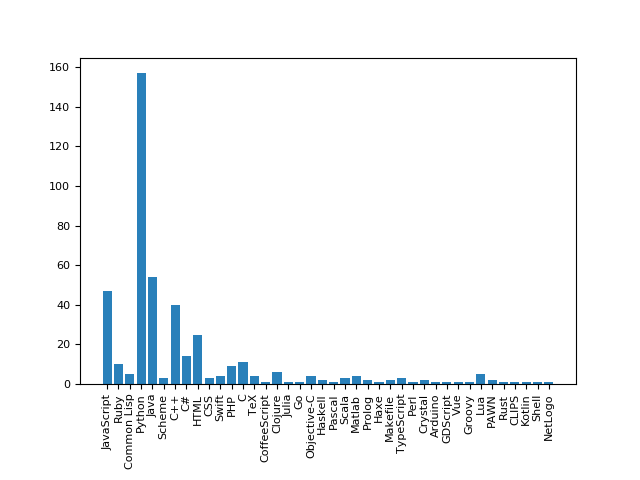
\includegraphics[width=1.0\textwidth]{imagenes/ai-lang.png}
    \caption{Número de proyectos por lenguaje entre los 500 proyectos de IA más populares de Github}
    \label{fig:ailang}
  \end{center}
\end{figure}

A priori parece que es cierto que hay lenguajes que destacan más en el campo de la inteligencia artificial, pero cabe la posibilidad de que estos datos simplemente reflejen la popularidad de cada lenguaje. Para descartar esto obtendremos los 500 repositorios más populares de GitHub y calcularemos el ratio de uso en IA frente al uso general de cada lenguaje:\\

\begin{lstlisting}[style=python, caption={Script para obtener el ratio entre proyectos de IA y proyectos generales por lenguaje en Github}]
# Obtenemos los 500 repositorios más populares de GitHub
popular_repos = itertools.islice(g.search_repositories("stars:>1", sort="stars"), 500)
popular_repos_by_lang = count_repos_by_lang(popular_repos)

# Calculamos el ratio de uso de cada lenguaje en proyectos de ia y en general
proportion_by_lang = {}
for lang in ai_repos_by_lang.keys():
	proportion_by_lang[lang] = ai_repos_by_lang[lang] / popular_repos_by_lang.get(lang, -1)

# Lo disponemos en una gráfica
plt.axes().yaxis.set_minor_locator(ticker.MultipleLocator(1))
plt.axhline(y=0, linewidth=0.75, color=(0.27, 0.27, 0.27))
plt.axhline(y=1, linewidth=0.35, color=(0.27, 0.27, 0.27))
plt.bar(list(proportion_by_lang.keys()), list(proportion_by_lang.values()), color=(0.16, 0.5, 0.73, 1))
plt.xticks(rotation=90, fontsize='8')
plt.yticks(fontsize='8')
plt.subplots_adjust(bottom=0.2)
plt.show()
\end{lstlisting}

Notar que si un lenguaje se ha usado en proyectos de IA pero no en proyectos generales el ratio sería infinito, en este caso le asignaremos como valor el número de repositorios de IA en el que se usa pero en negativo, para que no haya confusión. Teniendo esto en cuenta los resultados quedan como se muestra en la figura \ref{fig:proplang}.\\

\begin{figure}[h]
  \begin{center}
    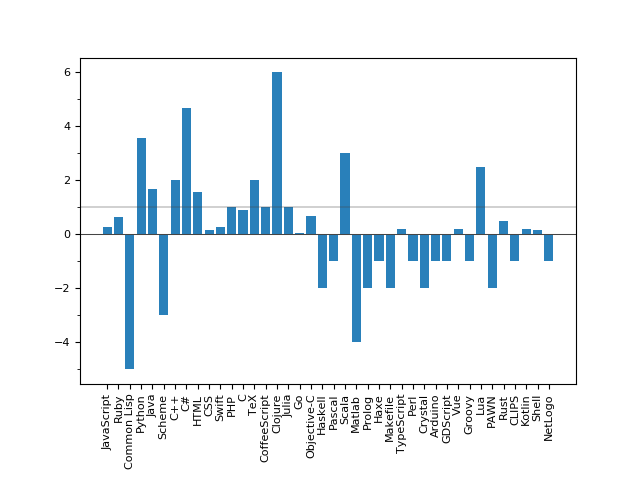
\includegraphics[width=1.0\textwidth]{imagenes/proportion-lang.png}
    \caption{Ratio entre proyectos de IA y proyectos generales por lenguaje en Github.}
    \label{fig:proplang}
  \end{center}
\end{figure}

Los lenguajes con un ratio menor que 1 son menos usados en IA que en otro tipo de proyectos y viceversa. Esto claramente no es un estudio serio, contiene bastantes errores que pueden arrojar datos imprecisos, por ejemplo depende de lo que GitHub entienda como ``artificial intelligence'' en su búsqueda. Además los ratios de algunos lenguajes pueden explicarse por sus particularidades, por ejemplo HTML y CSS, siendo lenguajes específicos del diseño web, es esperable que no puntúen muy bien. Sin embargo creo que cumple con la intención de señalar que realmente hay lenguajes que atraen a los desarrolladores de IA más que otros. Entonces cabe preguntarse ¿por qué? Estas diferencias pueden deberse a múltiples factores: librerías, comunidad, soporte de herramientas (p.e. debuggers, gestores de paquetes), tradición, etc. Sin embargo estos elementos tienen que formarse alrededor de un lenguaje, por lo tanto este tiene que ofrecer un potencial que otros no, pero además esto nos lleva a otro punto a favor de un lenguaje especializado en IA.\\

Que un lenguaje esté especializado en inteligencia artificial no solo significa que adapte su sintaxis o que tenga determinados constructos semánticos especialmente útiles (lo cual no es poca cosa), significa que gran parte del esfuerzo estará dirigido a tener un entorno lo más adaptado posible. Significa que se podrán invertir recursos en tener las mejores librerías de NPL, ML, planificación, estadística, etc posibles. Que las herramientas tales como debuggers estarán pensadas especialmente para resolver los problemas que plantee este campo sin dividir recursos en las necesidades que puedan surgir de, por ejemplo, la programación web o la de sistemas. También quiere decir que todas estas herramientas y librerías podrían estar al día de los últimos avances en investigación. En definitiva, una menor superficie nos permite enfocar mejor nuestros esfuerzos.\\


\section{Cómo diseñar un lenguaje orientado a la IA}
Que un lenguaje para IA tenga sentido no quiere decir que las objeciones planteadas arriba estén erradas, ciertamente el hecho de que la inteligencia artificial como campo esté muy pobremente definido y que se mueva muy rápido plantea muchas dificultades.\\

Por estas razones no es factible que este lenguaje sea un \acs{DSL}, como podría serlo uno orientado a un dominio más concreto (p.e. \textit{Prolog} en programación lógica), sino que deberá ser un lenguaje de propósito general, pero con ciertas características especialmente convenientes.
El ejemplo más próximo sería trasladar lo que ha hecho \textit{Julia} en el área de la computación numérica a la inteligencia artificial.
Para extraer estas características primero debemos conocer las necesidades más habituales a la hora de implementar una IA.\\

\subsection{Peculiaridades de la inteligencia artificial como ingeniería de software}
Günter Neumann en \cite{neumann_programming_nodate} rescata ciertos elementos que diferencian el trabajo en inteligencia artificial del de otras áreas y que explicarían porqué \textit{Lisp} y \textit{Prolog} han sido lenguajes tan relevantes en este campo:\\

\begin{itemize}
  \item La IA se centra en la computación simbólica más que en el procesamiento de números, siendo especialmente adecuados para el manejo de símbolos los lenguajes declarativos.\\
  
  \item La especificación inicial de un problema de IA es compleja, es más eficaz desarrollar los algoritmos de forma gradual mediante prototipos.\\
  
  \item Los algoritmos de IA no requieren de un control total de la máquina, por lo que es beneficioso un mayor nivel de abstracción que libere al programador de detalles de bajo nivel como el manejo de memoria.\\
\end{itemize}

Aunque algunos de estos puntos ya han sido superados y los vemos como normales en los lenguajes actuales (incluso se podría discutir el primero dada la importancia de la estadística en la IA moderna), hay que tener en cuenta que antes de que \textit{Lisp} introdujese avances como la recolección de basura lo mejor que se tenía era \textit{Fortran}, que se especializaba en el puro procesamiento numérico.\\

Nos permitiremos añadir otros factores que, con base en la teoría computacional de la mente explicada de forma muy accesible por Steven Pinker en \textit{How the Mind Works} \cite{how_mind_works} y por experiencia personal, en nuestra opinión también caracterizan al campo:\\

\begin{itemize}
  \item Mayor énfasis en los algoritmos que en el diseño de software.
  
  \item Ejecuciones largas, se necesita algún mecanismo que asegure que el programa no va a fallar después de varias horas de ejecución por escribir mal el nombre de una variable.
  
  \item Consumo de recursos considerable.
  
  \item Uso de herramientas lógicas y estadísticas, siendo particularmente útil la capacidad de codificar objetivos y modelos del mundo.
  
  \item Frecuente manejo de diferentes estructuras de datos.
  
  \item Concurrencia. Muchos de nuestros procesos mentales ocurren en paralelo.
  
  \item Necesidad de feedback continuo. Esto ayuda en el proceso de ensayo y error que supone calibrar un algoritmo.
  
  \item Visualización y comparación de resultados.
  
  \item Diseño modular que facilite la integración de distintas herramientas de forma organizada.
\end{itemize}


Creemos que un lenguaje que de respuesta a estas particularidades es un buen candidato para ser usado en IA más allá de las diferentes modas que puedan sucederse.


\section{Aspectos principales de nuestro lenguaje}
Intentemos esbozar los principales componentes de un lenguaje pensando en dar solución a los puntos anteriores.

Parece buena idea establecer una lista de prioridades en características que puedan estar en conflicto. Esto permite simplificar la elección de introducir o no un elemento que requiere un ``trade-off'' entre alguna de estas. Basta ver si la característica que se beneficia tiene más prioridad que la que sale perjudicada. Para este caso la siguiente lista me parece razonable:

\begin{enumerate}
  \item Velocidad de implementación, testeo y cambio.
  
  \item Eficiencia.
  
  \item Corrección de los programas.
\end{enumerate}


\subsection{Runtime}
\subsubsection*{Sistema de traducción: Compilado AOT vs Interpretado vs JIT}
Veamos las ventajas e inconvenientes de cada uno de los tipos.\\

\textbf{Compilación AOT:}\\

\begin{itemize}
  \item {\color{okgreen} Ventaja}: Produce código muy eficiente.\\
  \item {\color{okgreen} Ventaja}: Solo pasa por el proceso de traducción una vez.\\
  \item {\color{okgreen} Ventaja}: Quien recibe el ejecutable no necesita tener un compilador instalado.\\
  \item {\color{myred} Inconveniente}: Cada vez que se quiera probar un cambio hay que volver a compilar. Puede paliarse con un buen sistema de compilación.\\
\end{itemize}

\textbf{Interpretación:}\\

\begin{itemize}
  \item {\color{okgreen} Ventaja}: Mayor flexibilidad (p.e. pueden modificarse a si mismos en tiempo de ejecución).\\
  \item {\color{okgreen} Ventaja}: No hay que compilar cada cambio.\\
  \item {\color{myred} Inconveniente}: Tiene más limitaciones a la hora de hacer eficiente el código.\\
  \item {\color{myred} Inconveniente}: Pasa por el proceso de traducción cada vez que se ejecuta el programa.\\
\end{itemize}

\textbf{Compilación JIT:}\\

\begin{itemize}
  \item {\color{okgreen} Ventaja}: Mantiene todas las ventajas de la interpretación.\\
  \item {\color{okgreen} Ventaja}: La eficiencia es cercana a la de la compilación AOT, incluso en algunos casos puede hacer optimizaciones específicas con los datos de la ejecución actual y los del entorno donde se ejecuta.\\
  \item {\color{myred} Inconveniente}: La compilación se realiza en cada ejecución.\\
  \item {\color{myred} Inconveniente}: Algunas optimizaciones que realizaría un compilador AOT son demasiado costosas para ser hechas en tiempo de ejecución.\\
  \item {\color{myred} Inconveniente}: Es complicado de implementar comparado con la interpretación y la compilación AOT. 
\end{itemize}

En nuestra opinión, el sistema que mejor cumple nuestros requisitos sería un compilador JIT con opción de compilación AOT. De esta forma conseguimos un workflow ágil con bastante eficiencia y en caso de que el overhead del JIT no sea aceptable o se necesite un ejecutable independiente se podría compilar AOT.
La principal desventaja sería la dificultad de implementación, que ya de por sí es elevada con un solo traductor (sobre todo en el caso de un JIT).


\subsubsection*{Manejo de memoria: manual vs GC vs ownership}

\textbf{Manual:}\\

\begin{itemize}
  \item {\color{okgreen} Ventaja}: Control total sobre la memoria, lo que permite programas más eficientes. \\
  \item {\color{myred} Inconveniente}: El programador debe razonar sobre la memoria, lo cual consume ``espacio cognitivo'' para pensar en los algoritmos.\\
  \item {\color{myred} Inconveniente}: Es un sistema propenso a fallos que además no pueden detectarse en tiempo de compilación (El lenguaje no es seguro).\\
\end{itemize}

\textbf{Recolector de basura:}

\begin{itemize}
  \item {\color{okgreen} Ventaja}: El programador se despreocupa del manejo de la memoria.\\
  \item {\color{okgreen} Ventaja}: Permite lenguajes seguros.\\
  \item {\color{myred} Inconveniente}: Añade overhead a la ejecución.\\
  \item {\color{myred} Inconveniente}: Aumenta la complejidad del compilador.\\
\end{itemize}

\textbf{Ownership (à la \textit{Rust}):}

\begin{itemize}
  \item {\color{okgreen} Ventaja}: Permite lenguajes seguros, los fallos de memoria se detectan en tiempo de compilación.\\
  \item {\color{okgreen} Ventaja}: No añade overhead.\\
  \item {\color{myred} Inconveniente}: El programador sigue teniendo que razonar sobre la memoria, además con restricciones sobre su uso.\\
\end{itemize}

Dado que tanto el manejo manual como el ownership distraen al programador de su tarea principal y dificultan el realizar cambios en el código, siguiendo nuestra lista de prioridades la única opción factible que nos queda es usar un recolector de basura.\\


\subsection{Sistema de tipos}
La primera elección que tenemos que tomar claramente es si queremos un sistema de tipos, es decir, si nuestro lenguaje va a ser débilmente o fuertemente tipado.\\

Un sistema débil proporciona más flexibilidad y rapidez en la implementación, pero uno fuerte da herramientas para asegurar cierto buen comportamiento de los programas y la información extra puede aprovecharse para generar código más eficiente.\\

Por suerte existe una forma de obtener las ventajas de ambos sistemas, el tipado gradual. Un lenguaje con este sistema permitiría prototipados que pueden cambiarse rápidamente y una vez que se ha llegado a una versión definitiva poder garantizar cierta corrección. Me parece el sistema ideal a la hora de trabajar en algoritmos de inteligencia artificial.\\


\subsection{Concurrencia}
La capacidad de paralelizar código es crucial en el ámbito de la IA, no solo porque permite disminuir el tiempo de ejecución de los programas, sino porque es muy posible que la inteligencia real esté constituida de muchos procesos que trabajan a la vez, en palabras de Marvin Minsky ``la mente es una sociedad de agente''.\\

Siguiendo el razonamiento de liberar al programador de carga extra en la medida de lo posible, los sistemas de memoria compartida mediante mutex o semáforos quedan descartados. Esto nos deja con un sistema de paso de mensajes, mucho más simple y seguro.\\

En este aspecto es interesante la programación concurrente tipada, especialmente diseñada para paso de mensajes y que podría añadir una capa más de corrección al código. Sin embargo, como cualquier otro sistema de tipos, también resta flexibilidad y no conocemos ningún sistema de session-types graduales.\\


\subsection{Características finales}

Después de las consideraciones anteriores, y teniendo en cuenta las limitaciones de este trabajo, llegamos a la conclusión de que nuestro lenguaje debe ser compilado AOT, con recolección de basura, tipos graduales, facilidades al cálculo numérico como álgebra lineal incorporada en la sintaxis y a la computación simbólica como ``variants'' y átomos. Otros elementos también muy importantes, como la concurrencia y un sistema de módulos, se dejarán como trabajo futuro en pos de enfocarnos en mayor medida en el diseño de un sistema de tipos robusto.\\
